\begin{figure}[!h]
\centering
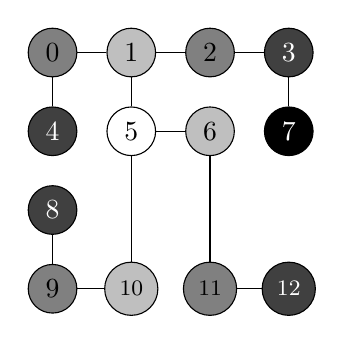
\begin{tikzpicture}[scale=1, label1/.style = {circle,fill=black!0,draw}, label2/.style = {circle,fill=black!25,draw}, label3/.style = {circle,fill=black!50,draw}, label4/.style = {circle,fill=black!75,draw, text=white}, label5/.style = {circle,fill=black!100,draw, text=white}, edge/.style = {-,thin}]
% vertex
\node[label1] (n5) at (2,3) {5};
\node[label2] (n10) at (2,1) {\footnotesize10};
\node[label2] (n1) at (2,4) {1};
\node[label2] (n6) at (3,3) {6};
\node[label3] (n9) at (1,1) {9};
\node[label3] (n11) at (3,1) {\footnotesize11};
\node[label3] (n0) at (1,4) {0};
\node[label3] (n2) at (3,4) {2};
\node[label4] (n8) at (1,2) {8};
\node[label4] (n4) at (1,3) {4};
\node[label4] (n12) at (4,1) {\footnotesize12};
\node[label4] (n3) at (4,4) {3};
\node[label5] (n7) at (4,3) {7};
%edges
\draw[edge] (n5) to (n1);
\draw[edge] (n5) to (n6);
\draw[edge] (n5) to (n10);
\draw[edge] (n1) to (n0);
\draw[edge] (n1) to (n2);
\draw[edge] (n10) to (n9);
\draw[edge] (n6) to (n11);
\draw[edge] (n0) to (n4);
\draw[edge] (n9) to (n8);
\draw[edge] (n2) to (n3);
\draw[edge] (n11) to (n12);
\draw[edge] (n3) to (n7);
\end{tikzpicture}
\caption{Ejemplo de búsqueda en anchura}
Dado un grafo conexo no direccionado, se realiza la búsqueda en anchura en $s=5$, obteniendo el siguiente el recorrido Capa 0: 5; Capa 1: 1,6,10; Capa 2: 0,2,11,9; Capa 3: 4,3,12,8 y Capa 4: 7. \\Fuente: \cite{Halim2019}.
\label{ejemBfs}
\end{figure}